\chapter{Cyclic Counting}

\section{Hemachandra Wheels}

In \zcref{section:hemachandra} we considered the problem of counting the number $H_n$ of ways we can subdivide a strip of $n$ blocks into squares and dominoes. An equivalent formulation of this problem was stated \zcref{exercise:hemachandra-variant}, where the task was to find a recursive expression for the number of ways in which we could color some squares along a strip of length $n$ blue, so that no two blue squares are adjacent; this number is $H_{n+1}$. The same questions can also be asked for cycles instead of strips.

\begin{definition}
  A \define{Hemachandra wheel} of order $n$ is an $n$-element cyclic set in which the elements are colored white and blue, so that no two adjacent elements are both colored blue. Two Hemachandra wheels are considered to be the same when one can be obtained from the other by rotation. Elements of Hemachandra wheels will be called \define{segments}.

  A Hemachandra wheel is said to be \define{labeled} if its $n$ elements are labeled $0$ through $n-1$ in cyclic ordering. Two labeled Hemachandra wheels of order $n$ are considered to be the elements with matching labels have the same color.

  We write $W_n$ for the number of labeled Hemachandra wheels of order $n$, and we write $\tilde{W}_n$ for the number of (unlabeled) Hemachandra wheels of order $n$.
\end{definition}

\begin{figure}[t]
  \centering
    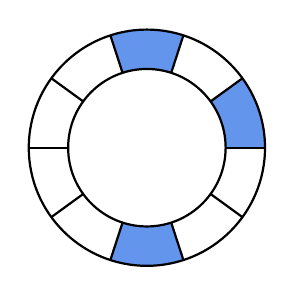
\begin{tikzpicture}
      \def\rin{1.0}
      \def\rout{1.5}
      \def\n{10}
      \pgfmathsetmacro{\step}{360/\n}
      
      \foreach \k in {0,2,7} {
        \fill[CornflowerBlue]
        (\k*\step:\rin)
        arc[start angle=\k*\step, end angle={(\k+1)*\step}, radius=\rin]
        -- ({(\k+1)*\step}:\rout)
        arc[start angle={(\k+1)*\step}, end angle=\k*\step, radius=\rout]
        -- cycle;
      }
      
      \draw[thick] (0,0) circle[radius=\rin];
      \draw[thick] (0,0) circle[radius=\rout];
      
      \foreach \a in {0,\step,...,324} {
        \draw[thick] (\a:\rin) -- (\a:\rout);
      }
    \end{tikzpicture}
  \caption[Hemachandra wheels]{Hemachandra wheels.}
  \label{figure:hemachandra-wheel}
\end{figure}

\begin{remark}
  The number $W_n$ of labeled Hemachandra wheels can be determined by considering two cases: Either the element labeled $0$ is white or it is blue. In the first case, the remaining elements of the Hemachandra wheel form a strip of elements labeled $1$ through $n-1$, and the number of colorings of this strip is $F_{n+1}$. In the second case, the blue element labeled $0$ cannot have an adjacent blue element, so the coloring of the remaining strip is determined by the coloring of the elements $2$ through $n-2$. Their number is $F_{n-1}$. Therefore, we conclude that
  \begin{equation*}
    W_n=F_{n+1}+F_{n-1}.
  \end{equation*}
  Since $F_{n+1}+F_{n-1}$ is the $n$\supth{} Lucas number $L_n$, we find that $W_n=L_n$.
\end{remark}

\begin{theorem}
  Consider the Fibonacci numbers $F_n$, and let $p$ be a prime number.
  \begin{equation*}
    \tilde{W}_p=\frac{1}{p}(F_{p+1}+F_{p-1}+p-1)
  \end{equation*}
\end{theorem}

\begin{proof}
  All labelings of the entirely white Hemachandra wheel are the same, so it corresponds to exactly one labeled wheel. Every wheel with at least one blue segment has $p$ distinct labelings. Indeed, if this were not so then its coloring would be preserved by a rotation through $k$ positions for some $0<k<p$. Since $p$ is prime, the positions $0,k,2k,\ldots,(p-1)k$ exhaust the wheel. Every position would therefore have the same color, a contradiction. Consequently, we have
  \begin{equation*}
    W_p=1+p(\tilde{W}_p-1),
  \end{equation*}
  and the result follows.
\end{proof}

\begin{corollary}\label{corollary:congruence-lucas-numbers-mod-p}
  For any prime number $p$ we have the congruence
  \begin{equation*}
    F_{p-1}+F_{p+1}\equiv 1\pmod{p}.
  \end{equation*}
\end{corollary}

\begin{proof}
  The number $\tilde{W}_p$ is an integer, so $p\mid F_{p+1}+F_{p-1}-1$.
\end{proof}

In many cases, our main method to prove congruences is by algebraic manipulation. In the previous theorem we found a new source of congruences: \emph{rotational symmetry!} In the present chapter we will refine this method and find many congruences that can be proven naturally with rotational symmetry.

\section{The Prime--Fixed Point Congruence}

\begin{definition}
  Consider a map $f:X \to X$. Then we define the set of \define{fixed points} of $f$ by
  \begin{equation*}
    \mathrm{Fix}(f):= \{x\in X\mid f(x)=x\}.
  \end{equation*}
\end{definition}

\begin{theorem}[The Prime--Fixed Point Congruence]\label{theorem:prime-fixed-point-congruence}
  Consider a finite set $X$ and a map $f:X\to X$ such that $f^p(x)=x$ for all $x\in X$, where $p$ is a prime number. Then we have
  \begin{equation*}
    |X| \equiv |\mathrm{Fix}(f)| \pmod{p}.
  \end{equation*}
  In particular, if $|X| \nequiv 0\pmod{p}$ and $f^p(x)=x$ for all $x\in X$, then $f$ has a fixed point.
\end{theorem}

\begin{proof}
  If $f(x)\neq x$, then the least positive $n$ for which $f^n(x)=x$ is $p$. Indeed, by the assumption that $p$ is prime, if $1<n<p$ then there is an integer $k$ such that $kn\equiv 1\pmod p$. For such $k$ we find that $f(x)=f^{kn}(x)=x$, contradicting our assumption on $x$. Thus we see that $X$ is partitioned into orbits of size $1$ and of size $p$, and the claim follows.
\end{proof}

\begin{example}
  The congruence of \zcref{corollary:congruence-lucas-numbers-mod-p} is an instance of \zcrefnamed{theorem:prime-fixed-point-congruence}, since the total number of Hemachandra wheels of order $p$ is
  \begin{equation*}
    F_{p-1}+F_{p+1},
  \end{equation*}
  and the only fixed point under rotation is the entirely white Hemachandra wheel.
\end{example}

Solomon Golomb used the prime--fixed point congruence to one of the most fundamental results of elementary number theory, Fermat's Little Theorem \cite{golomb1956}. This theorem is of such importance, that we will prove it here and again in the next chapter, where we will explore its consequences.

\begin{theorem}[Fermat's Little Theorem---Combinatorial Version]\label{theorem:fermats-little-theorem-combinatorial}
  Consider a prime number $p$ and an integer $a$. Then the congruence
  \begin{equation*}
    a^{p}\equiv a\pmod{p}
  \end{equation*}
  holds.
\end{theorem}

\begin{figure}[t]
  \centering
  \begin{minipage}{0.45\textwidth}
    \centering
    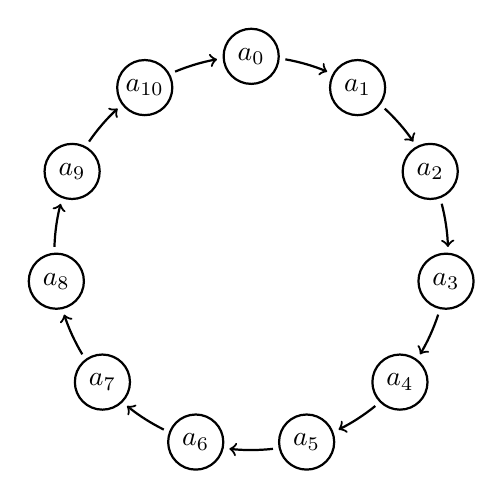
\begin{tikzpicture}[
      thick,
      every node/.style={circle, draw, minimum size=7mm, inner sep=1pt}
      ]
      \def\n{11}
      \def\radius{2.5cm}
      
      \foreach \i in {1,...,\n} {
        \pgfmathsetmacro{\value}{int(\i-1)}
        \node (N\i) at ({90-360/\n*(\i-1)}:\radius) {$a_{\value}$};
      }
      
      \foreach \i in {1,...,\n} {
        \pgfmathsetmacro{\angle}{90-360/\n*(\i-1)}
        \draw[->]
        (\angle-10:\radius)
        arc[start angle=\angle-10,
        delta angle=-360/\n+20,
        radius=\radius];
      }
    \end{tikzpicture}
  \end{minipage}
  \hfill
  \begin{minipage}{0.45\textwidth}
    \centering
    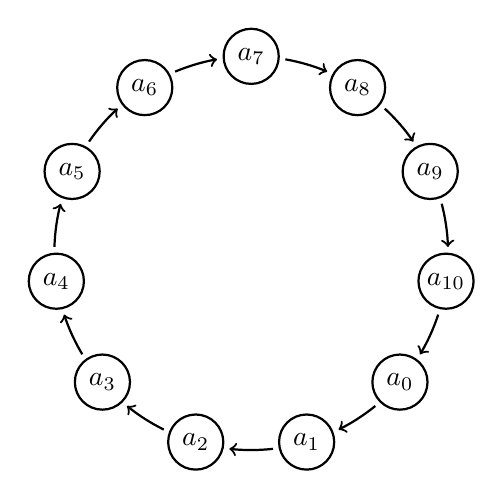
\begin{tikzpicture}[
      thick,
      every node/.style={circle, draw, minimum size=7mm, inner sep=1pt}
      ]
      \def\n{11}
      \def\radius{2.5cm}
      
      \foreach \i in {1,...,\n} {
        \pgfmathsetmacro{\value}{int(mod(\n+\i-5,\n))}
        \node (N\i) at ({90-360/\n*(\i-1)}:\radius) {$a_{\value}$};
      }
      
      \foreach \i in {1,...,\n} {
        \pgfmathsetmacro{\angle}{90-360/\n*(\i-1)}
        \draw[->]
        (\angle-10:\radius)
        arc[start angle=\angle-10,
        delta angle=-360/\n+20,
        radius=\radius];
      }
    \end{tikzpicture}
  \end{minipage}
  
  \caption[Golomb's proof of Fermat's Little Theorem]{%
    \label{figure:golombs-proof-FLT}%
    In Golomb's proof of Fermat's Little Theorem, two labellings of a
    cyclic set $C$ with elements from a set $A$ are considered the
    same, or equivalent, if one can be obtained from the other by
    rotation.%
  }
\end{figure}

\begin{proof}[Golomb's combinatorial proof]
  Consider a set $A$ with $a$ elements, and a cyclic set $C$ with $p$ elements. Then there are $a^p$ functions from $C$ to $A$, which we view as labellings of the elements of $C$. The fixed points under rotation are precisely the labellings defined by a constant function $C\to P$. The number of such constant functions is $a$. Therefore it follows by \zcref{theorem:prime-fixed-point-congruence} that
  \begin{equation*}
    a^p\equiv p \pmod{p}.\qedhere
  \end{equation*}
\end{proof}

\section{Lucas's Theorem}

Our next application of \zcref{theorem:prime-fixed-point-congruence} is a theorem due to {\'E}douard Lucas \cite{lucas1878congruences}, which allows us to compute the residue class of binomial coefficients modulo a prime. This theorem is complementary to \zcrefnamed{theorem:kummers-theorem}, which gives a complete description of the prime factorization of binomial coefficients. The proof we present below is due to Bruce Sagan \cite[Theorem 6.5.6]{sagan2020}.

\begin{theorem}[Lucas's Theorem]
  Consider a prime number $p$, and natural numbers $m$ and $n$ written in base $p$ as
  \begin{equation*}
    m=\sum_{i=0}^ka_ip^i\qquad\text{and}\qquad n=\sum_{i=0}^kb_ip^i.
  \end{equation*}
  Then the congruence
  \begin{equation*}
    \binom{n}{m}\equiv\prod_{i=0}^k\binom{b_i}{a_i}\pmod{p}
  \end{equation*}
  holds. In particular, if $b_i<a_i$ for some $i$, then $\binom{n}{m}$ is divisible by $p$.
\end{theorem}

\begin{proof}
  By Euclidean division, write $m= rp+a_0$ and $n=sp+b_0$, so that 
  \begin{equation*}
    r=\sum_{i=0}^{k-1}a_{i+1}p^i\qquad\text{and}\qquad s=\sum_{i=0}^{k-1}b_{i+1}p^i
  \end{equation*}
  It suffices to show that
  \begin{equation*}
    \binom{n}{m}\equiv \binom{s}{r}\binom{b_0}{a_0}\pmod{p},
  \end{equation*}
  since the claim follows by iterating this congruence. Consider an $n$-element set $X$ and a map $f:X\to X$ so that the number of $p$-cycles is $s$ and the number of fixed points is $b_0$. Then we can define a map $\varphi$ on the set of $m$-element subsets of $X$ by
  \begin{equation*}
    \varphi(U):=\{f(x)\mid x\in U\}.
  \end{equation*}
  The image of an $m$-element subset $U$ under $f$ is indeed again an $m$-element subset. Furthermore, since $f$ satisfies $f^p(x)=x$ for all $x\in X$, it also follows that $\varphi^p(U)=U$ for every $m$-element subset of $X$. Therefore it follows by \zcref{theorem:prime-fixed-point-congruence} that
  \begin{equation*}
    \binom{n}{m}\equiv |\mathrm{Fix}(\varphi)|\pmod{p}.
  \end{equation*}
  Now observe that $\varphi(U)=U$ if and only if for every $x\in U$ we have $f(x)\in U$. This means that for every $x\in U$, the entire orbit under $f$ is contained in $U$. As we have seen in \zcref{theorem:prime-fixed-point-congruence}, these orbits have either $p$ elements or $1$ element. Since the number of fixed points of $f$ is $0\leq b_0<p$, it follows that every $m$-element subset contains of a number $t$ of orbits with $p$ elements, and a number $0\leq c<p$ of fixed points, which allows us to write $m=tp+c$. By the uniqueness property of \zcrefnamed{theorem:euclidean-division}, it follows that $t=r$ and $c=a_0$. We conclude that a fixed point $U$ of $\varphi$ consists of a choice of $r$ orbits with $p$ elements and a choice of $a_0$ fixed points of $f$, so that
  \begin{equation*}
    |\mathrm{Fix}(\varphi)|=\binom{s}{r}\binom{b_0}{a_0}.\qedhere
  \end{equation*}
\end{proof}

\section{The Orbit--Counting Formula}

\begin{definition}
  Consider a finite set $X$ and a bijection $f:X\to X$. We say that two elements $x$ and $y$ of $X$ lie \define{in the same orbit} of $f$ if there exist a natural number $k$ such that
  \begin{equation*}
    f^k(x)=y.
  \end{equation*}
\end{definition}

\begin{proposition}
  The relation $x\sim y$ of lying in the same orbit of a bijection $f$ is an equivalence relation.
\end{proposition}

\begin{proof}
  To see that the relation $\sim$ is reflexive, note that $f^0(x)=x$. To see that the relation $\sim$ is transitive, suppose that $f^k(x)=y$ and $f^l(y)=z$. Then it follows that $f^{k+l}(x)=z$.

  The proof that the relation $\sim$ is symmetric is slightly more work. Let $k$ be the least natural number such that $f^k(x)=y$, and consider the infinite sequence
  \begin{equation*}
    x,~f(x),~f^2(x),~\ldots
  \end{equation*}
  Since the set $X$ is assumed to be finite, there must exist a least positive integer $m$ such that $f^m(x)=f^i(x)$ for some $0\leq i<m$. We claim that $i=0$. Indeed, if $0<i$, then the assumption that $f$ is a bijection implies the equation $f^{m-1}(x)=f^{i-1}(x)$, which contradicts the minimality of $m$. Thus the infinite sequence $(f^i(x))_{i\in\mathbb{N}}$ is periodic with period $m$. It follows that $k\leq m$, and that
  \begin{equation*}
    f^{m-k}(y)=f^{m-k}(f^k(x))=f^m(x)=x.
  \end{equation*}

  Then we have $f^l(y)=f^k(x)$, showing that $y\sim x$. Finally, to see that $\sim$ is transitive, suppose that $f^k(x)=f^l(y)$ and that $f^u(y)=f^v(z)$. Then we have
  \begin{equation*}
    f^{k+u}(x)=f^u(f^k(x))=f^u(f^l(y))=f^l(f^u(y))=f^l(f^v(z))=f^{l+v}(z).\qedhere
  \end{equation*}
\end{proof}

Since the relation $\sim$ is an equivalence relation, it follows that the equivalence classes of the relation $\sim$ partition the set $X$. The equivalence classes of this relation are called \define{orbits}. Recall from \zcref{exercise:orbit-order-theorem} that
\begin{equation*}
  f^k(x)=x\qquad\Leftrightarrow\qquad d\mid k.
\end{equation*}
That is, $x$ is a \emph{fixed point} of the map $f^k:X\to X$ if and only if $k$ is a multiple of the number of elements in the orbit of $x$. Fixed points play an essential role in the orbit--counting formula.

\begin{definition}
  Consider a map $f:X\to X$ on a finite set $X$. We write
  \begin{equation*}
    \nu_f(n):=|\mathrm{Fix}(f^n)|.
  \end{equation*}
\end{definition}

The following theorem is a special case of a more general theorem of group theory, called \emph{Burnside's Lemma}.

\begin{lemma}[The Orbit--Counting Formula]\label{theorem:orbit-counting}
  Consider a finite set $X$ and a map $f:X\to X$ such that $f^n(x)=x$ for all $x\in X$. Let $N$ be the number of orbits of $f$. Then we have
  \begin{equation*}
    N=\frac{1}{n}\sum_{k=0}^{n-1}|\mathrm{Fix}(f^k)|.
  \end{equation*}
\end{lemma}

\begin{proof}
  We will prove the equation
  \begin{equation*}
    nN=\sum_{k=0}^{n-1}|\mathrm{Fix}(f^k)|.
  \end{equation*}
  Note that $\sum\nolimits_{k=0}^{n-1}|\mathrm{Fix}(f^k)|$ is the number of elements in the set
  \begin{equation*}
    A:=\{(k,x) \mid f^k(x)=x\}\subseteq \{0,\ldots,n-1\}\times X.
  \end{equation*}
  Now consider an orbit $T$ of size $t$. Then it follows for each $x\in T$ that $f^k(x)=x$ if and only if $k$ is a multiple of $t$. In other words, for each $x\in T$ we have
  \begin{equation*}
    (k,x)\in A \Leftrightarrow t \mid k.
  \end{equation*}
  It follows that the set $\{(k,x)\in A\mid x\in T\}$ has size $\frac{n}{t}t=n$, and we conclude that $|A|$ is $n$ times the number of orbits of $f$.
\end{proof}

\begin{theorem}
    Consider a finite set $X$ and a map $f:X\to X$ such that $f^n(x)=x$ for all $x\in X$. Let $N$ be the number of orbits of $f$. Then we have
  \begin{equation*}
    N=\frac{1}{n}(\nu_f\ast \varphi)(n).
  \end{equation*}
\end{theorem}

\section{Cyclic Coloring}

\begin{theorem}
  Consider two natural numbers $1\leq k<n$, and let $g=\gcd(n,k)$. Define the function
  \begin{equation*}
    S(n,k)=-\sum_{\substack{d\mid g\\ d>1}}\mu(d)\binom{n/d}{k/d}.
  \end{equation*}
  Then we have
  \begin{equation*}
    n\mid \binom{n}{k}\quad\Leftrightarrow\quad n\mid S(n,k).
  \end{equation*}
\end{theorem}

\begin{proof}
  Consider a cyclic set $C$ of order $n$, and let $X$ be the set of all $k$-element subsets of $C$. The number of elements in $X$ is $\binom{n}{k}$. Let $U\subset X$ be the subset consisting of $k$-element subsets of $C$ that are invarant under rotation by $r$ steps for some $0<r<n$. Every $k$-element subset of $C$ outside of $U$ has $n$ distinct rotations. The set $X\setminus U$ is therefore partitioned into orbits of size $n$. Consequently, we obtain
  \begin{equation*}
    \binom{n}{k}\equiv \# U \pmod{n}.
  \end{equation*}
  It remains to show that $S(n,k)$ is the number of $k$-element subsets of $C$ in $U$.

  For each $d\mid n$, let $U_d$ be the collection of $k$-element subsets of $C$ that are invariant under rotation by $n/d$ steps. Note that a $k$-element subset of $C$ belongs to $U_d$ precisely when it is a union of orbits of the rotation by $n/d$ steps. Each such orbit contains exactly $d$ elements, so it follows that $U_d$ is empty unless $d\mid k$. When $d\mid k$, then a $k$-element subset invariant under rotation by $n/d$ steps is a $k/d$-element subset of such orbits. Therefore, we have
  \begin{equation*}
    \# U_d = \binom{n/d}{k/d}
  \end{equation*}
  for every divisor $d\mid g$. Note that $U_d\subseteq U_d'$ for every $1<d'\mid d$. Therefore it follows that
  \begin{equation*}
    U=\bigcup_{p\mid g} U_p.
  \end{equation*}
  It follows by \zcrefnamed{theorem:inclusion-exclusion-principle} that
  \begin{equation*}
    \# U=\sum_{p\mid g}\binom{n/p}{k/p}-\sum_{p<q\mid g}\binom{n/pq}{k/pq}+\cdots = -\sum_{d\mid g}\mu(d)\binom{n/d}{k/d}.\qedhere
  \end{equation*}
\end{proof}

\section{Cyclic Integer Partitions}

\section{Cyclic Lists}

\section{Cyclic Trees}

\begin{enumerate}
\item Count the number of trivalent trees with $n$ cyclically ordered leaves.
\item Count the number of rooted trivalent trees with $n$ cyclically ordered leaves.
\item Count the number of triangulations of the regular $n$-gon up to rotation.
\item Count the number of trees with $n$ cyclically ordered leaves, so that each node has degree $\geq 3$.
\item Count the number of rooted trees with $n$ cyclically ordered leaves, so that each node has degree $\geq 3$.
\item Count the number of bijections up to rotation on a cyclically ordered set with $n$ elements.
\item Count the number of transitive bijections up to rotation on a cyclically ordered set with $n$ elements.
\item Count, up to rotation, the number of functions $f:X\to X$ such that for each $x\in X$ the set $f^{-1}(x)$ is empty or has at least two elements, and the set $\{x\in X\mid f^{-1}(x)=\varnothing\}$ is cyclically ordered with $n$ elements.
\item Count the number $B_n$ of $2$-colorings of a wheel with $n$ beads up to rotation. Say that a $3$-coloring of a wheel is \define{proper} of no two adjacent beads are of the same color. Count the number $C_n$ of proper $3$-colorings of a necklace with $n$ beads up to rotation. Show that
  \begin{equation*}
    C_n =
    \begin{cases}
      B_n & \text{if $n$ is even,}\\
      B_n-2 & \text{if $n$ is odd.}
    \end{cases}
  \end{equation*}
  Answer: $C_n=\sum_{d\mid n}\varphi(n/d)(2^d+2(-1)^d)$.
\item Count the number of families of pairwise disjoint two-element subsets of beads of an $n$-cycle
\end{enumerate}

\exercises

\begin{routine}
  \exercise Let $n=mp^k$, where $p$ is a prime such that $p\nmid m$, and let $F$ be the sequence of Fibonacci numbers. Show that
  \begin{equation*}
    F_{n-1}+F_{n+1}\equiv F_{m-1}+F_{m+1}\pmod{p}.
  \end{equation*}
  \exercise Consider a prime $p$. Show that
  \begin{equation*}
    \binom{n}{m} \equiv \binom{n-p}{m-p}+\binom{n-p}{m}\pmod{p}.
  \end{equation*}
  \exercise Determine the number of labeled and unlabeled bicolored wheels with $n$ segments in which no three adjacent segments all have the same color.
\end{routine}

%%% Local Variables:
%%% mode: latex
%%% TeX-master: "number-theory"
%%% TeX-engine: luatex
%%% End:

